\documentclass[11pt]{article}
\usepackage[utf8]{inputenc}
\usepackage[english]{babel}
\usepackage{bilal2vec}

\title{SE 380 — HW 2}
\author{Bilal Khan\\
\href{mailto:bilal2vec@gmail.com}{bilal2vec@gmail.com}}
\date{\today}

\begin{document}

\maketitle

\tableofcontents

\section{1}

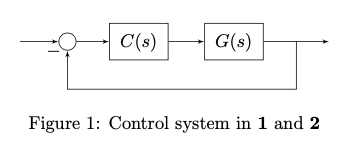
\includegraphics[width=200pt]{a4_1.png}

Consider the feedback control system where

\[ G(s) = \dfrac{5}{(1 + s) \left(1 + \dfrac{2 \zeta}{\omega_n} s + \dfrac{s^2}{\omega_n^2} \right)} \]

With $\omega_n = 10$ and $\zeta = 0.1$.

Design a controller $C(s)$ such that the closed-loop system has the following specifications: The steady state error in response to a unit step function is $e_\infty \leq 0.05$, the gain margin $k_m \geq 10$dB, and the phase margin $\phi_m \geq 60^\circ$.

We will design a controller with two parts: $C_1(s) = \mu / s^p$, to satisfy the steady state error requirement and we choose $p = 0$, and $C_2(s)$, to be a realizable controller that does not change the steady state behavior of the closed loop system to satisfy the gain and phase margin requirements.

\begin{align*}  
  y_\infty &= \dfrac{C_1(0)C_2(0)G(0)}{1 + C_1(0) C_2(0) C_3(0)} \\
  &= \dfrac{\mu * 1 * 5}{1 + \mu * 1 * 5} \\
  &= \dfrac{5 \mu}{1 + 5 \mu} \\
\end{align*}

For our steady state error requirement, we need $y_\infty \leq 0.05$, so manipulating this, we can see that we need $\mu \geq 3.8$. For simplicity, we choose $\mu = 4$.

For $C_2(s)$ to not change the steady state behavior of the closed loop system, we need $C_2(0) = 1$. We also need $C_2(s)$ to be realizable, so we choose to define it in the form $C_2(s) = \frac{L^\star(s)}{C_1(s) G(s)}$. The steady state gain of $G(s)$ is $5$, so we need $L^\star(0) = 5$. For the controller to be realizable, it must have the same degree as $G(s)$, 3. For a phase margin of at least $60^\circ$ and a gain margin of atleast $10$ dB, we will choose an arbitrary crossover point $\omega_c$ for the magnitude path of the bode plot of the controller to hit zero such that these two requirements are satisfied. We will choose $\omega_c = 10^1$ for simplicity (Any choice of $\omega_c$ will work). For the margins to be appropriately large, it is safe to place one pole at least one decade before $\omega_c$ and the other two poles at least one decade after $\omega_c$. 

\begin{align*}
  C_2(s) &= \dfrac{L^\star(s)}{C_1(s) G(s)} \\
  L^\star(s) &= \dfrac{5}{(1 + \frac{s}{10^0})(1 + \frac{s}{10^2})^2} \\
  C(s) &= C_1(s) C_2(s) \\
  &= C_1(s) L^\star(s) \dfrac{1}{G(s)} \\
  &= 4.0 \dfrac{5}{(1 + \frac{s}{10^0})(1 + \frac{s}{10^2})^2} \dfrac{(1 + s) \left(1 + \dfrac{2 \zeta}{\omega_n} s + \dfrac{s^2}{\omega_n^2} \right)}{5} \\
  &= 4.0 \cdot \dfrac{(1 + s) \left(1 + \dfrac{2 \zeta}{\omega_n} s + \dfrac{s^2}{\omega_n^2} \right)}{(1 + \frac{s}{10^0})(1 + \frac{s}{10^2})^2} \\
\end{align*}

In code, we can verify that the controller satisfies the requirements:

\inputminted{python}{a4_1.py}

$G(s)$ Bode Plot

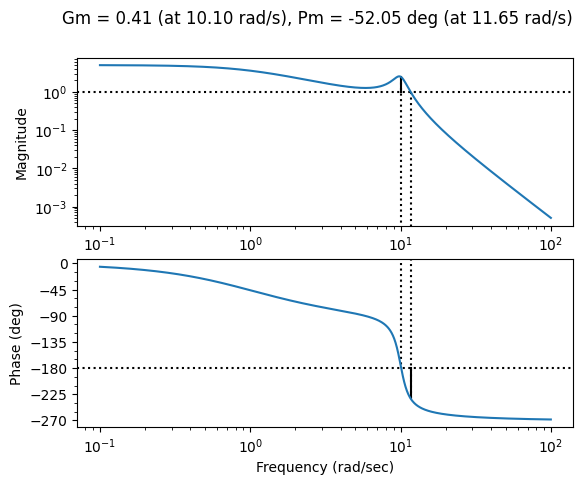
\includegraphics[width=200pt]{a4_2.png}
  
$G(s)$ Step Response

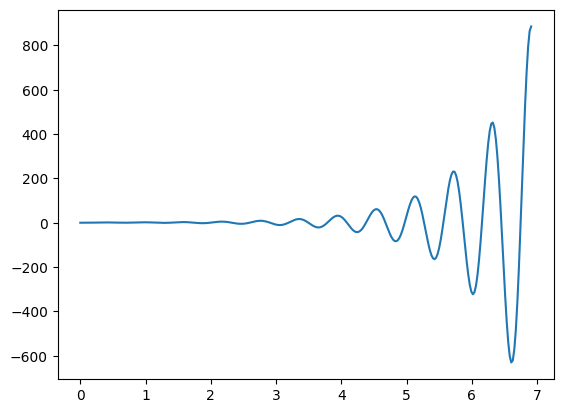
\includegraphics[width=200pt]{a4_3.png}

$C(s)$ Bode Plot

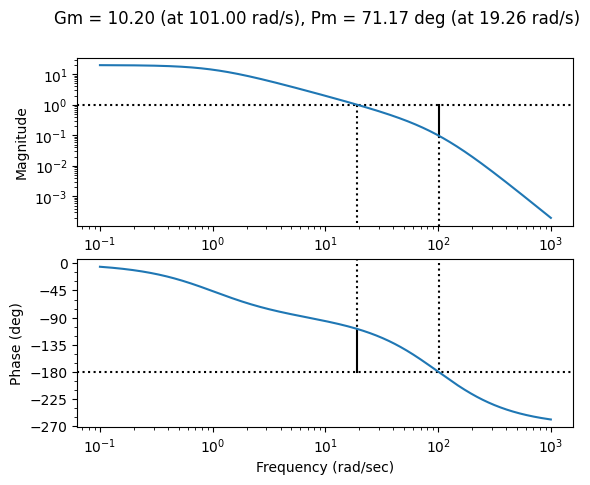
\includegraphics[width=200pt]{a4_4.png}
  
$C(s)$ Step Response

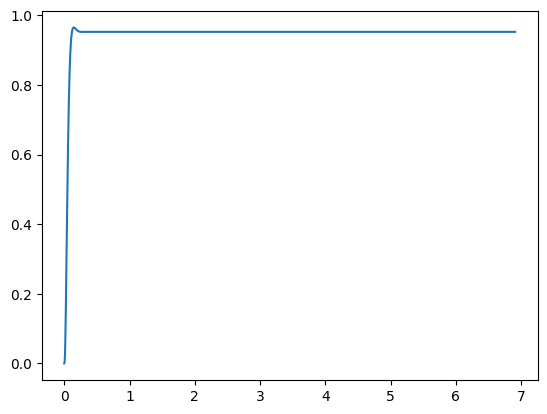
\includegraphics[width=200pt]{a4_5.png}

As we can see, the steady state error is less than $0.05$ (the output is $> 0.95$ at the end of the step response once the oscillations have settled), the gain margin is greater than $10$ dB, and the phase margin is greater than $60^\circ$.

\section{2}

For the same feedback control system as part 1, design a controller $C(s)$ such athat the closed-loop system has the following specifications: No overshoot, the settling time at $1\%$ is $T_s^{1\%} \leq 0.5\%$, and the steady-state error in response to a unit step function is $|e_\infty| = 0$.

To do this we will adapt the controller from part 1. The controller from part one consists of $C_1(s)$ which was used to control the steady-state error, and $C_2(s)$ which was used to make the system stable and satisfy the gain and phase margin requirements. We will keep $C_2(s)$ the same since we still want the controller to stabilize the system (satisfying the gain and phase margin requirements is an extra bonus to keep the system in a "safe" region of stability) and replace $C_1(s)$ with a controller that will make the system have no overshoot and a settling time of $0.5\%$. To do this we want to use a proportional-integral controller as it increases the steady state gain to zero error and only marginally reduces the phase margin.

\[ mu = 2 \cdot \alpha \]
\[ c = \dfrac{\mu}{\alpha} \]
\[ T = \dfrac{10}{\omega_c} \]
\[ C_3(s) = c + \dfrac{c}{T} \dfrac{1}{s} \]

We will keep $\alpha = 10$ and $T = 10 / \omega_c$ using our crossover $\omega_c$ value from part 1 to keep the phase margin decline limited to $\approx 6\%$. We decide to set our increase of the steady state gain to $\mu = 2 \cdot \alpha$ instead of $\alpha$ since the value reached the settling time requirement too slowly.

We can verify that the controller satisfies the requirements in code:

\inputminted{python}{a4_2.py}

As we can see the overshoot is zero (modulo floating point rounding issues at $\approx 1e-8$), the error after $t = 0.5$ stays at less that $0.1\%$ satisfying the settling time requirement, and the steady state error is zero (neglibly small at $\approx 1e-8$).

$G(s)$ Bode Plot

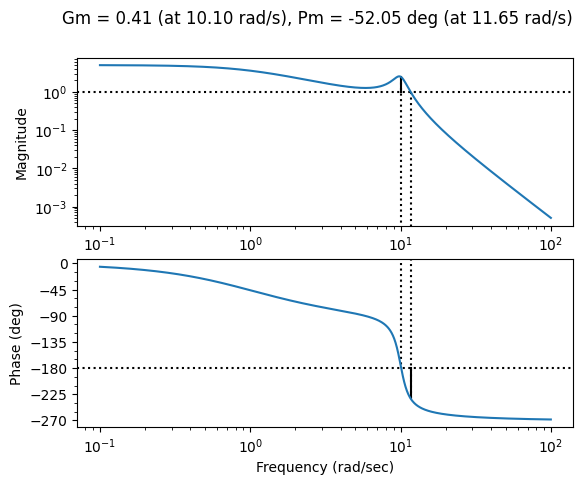
\includegraphics[width=200pt]{a4_6.png}
  
$G(s)$ Step Response

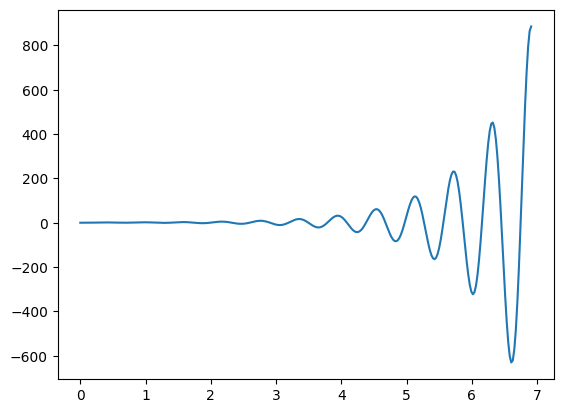
\includegraphics[width=200pt]{a4_7.png}

$C(s)$ Bode Plot

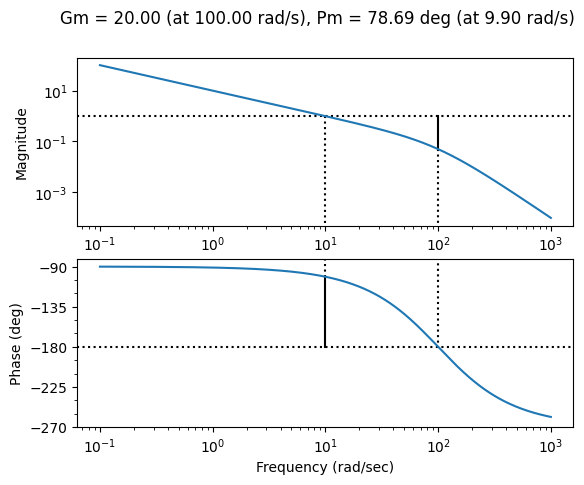
\includegraphics[width=200pt]{a4_8.png}
  
$C(s)$ Step Response

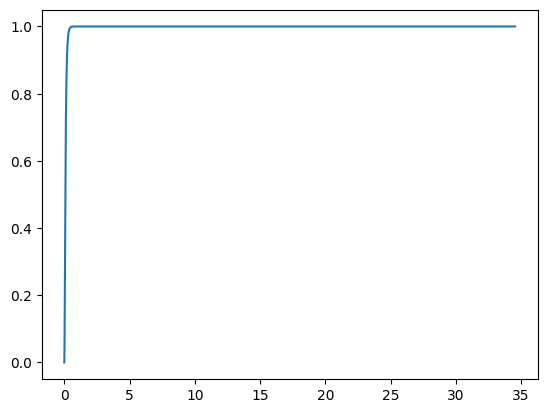
\includegraphics[width=200pt]{a4_9.png}

\end{document}
